\subsection{Общая сумма больше суммы выручки по ОРП}
%\marginnote{\Date{Чт.}{19}{Июл.}{2018}}[-40pt]

\begin{itemize}	
	\item Ситуация возникает, когда чек пробит, оплата произведена и чек ушел в ОФД, но отсутствует в 1С.

	
	\begin{figure}[H]
		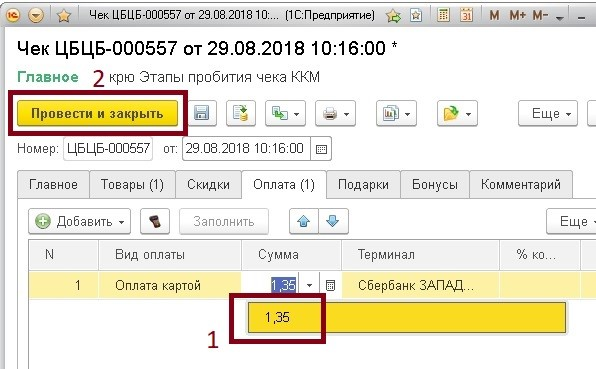
\includegraphics[width=1.0\textwidth]{12.jpg}
		\caption{<<Потерянный чек>>.}
		\label{ris:12.jpg}
	\end{figure}
	Здесь видно, что общая сумма  на 100 р. больше суммы выручки по ОРП.  (Рис.~\ref{ris:12.jpg})
	\item Первое, что  необходимо сделать - проверить по бумажным отчетом, что суммы внесены правильно. И если это действительно так и есть расхождения чисел, а не допущена ошибка ввода, приступаем к поискам потерянного чека.
	Нужно путем опроса кассиров или поиском в ОФД способом выяснить, какой товар был в этом чеке. . (Работа с сайтом ОФД изложена в п. \ref{5500})
	
	
	Установив товар в чеке или приняв решение чем его заменить нам нужно добавить этот чек в ОРП. Как  это сделать:
	
	\begin{itemize}
		\item Создать чек по нужной кассе. Записать его и с помощью ИТ отдела пересобрать ОРП.
		      Таким образом сумма выручки по ОРП сравняется с суммой по Z-отчету
	\end{itemize}
	
	
	
\end{itemize}
